\documentclass[
11pt, % The default document font size, options: 10pt, 11pt, 12pt
%codirector, % Uncomment to add a codirector to the title page
]{charter} 

\usepackage{subfig}


% El títulos de la memoria, se usa en la carátula y se puede usar el cualquier lugar del documento con el comando \ttitle
\titulo{Autoencoders para reforzar modelos de prevención de fraude} 

% Nombre del posgrado, se usa en la carátula y se puede usar el cualquier lugar del documento con el comando \degreename
%\posgrado{Carrera de Especialización en Sistemas Embebidos} 
%\posgrado{Carrera de Especialización en Internet de las Cosas} 
\posgrado{Carrera de Especialización en Inteligencia Artificial}
%\posgrado{Maestría en Sistemas Embebidos} 
%\posgrado{Maestría en Internet de las cosas}

% Tu nombre, se puede usar el cualquier lugar del documento con el comando \authorname
\autor{Ariel Salassa} 

% El nombre del director y co-director, se puede usar el cualquier lugar del documento con el comando \supname y \cosupname y \pertesupname y \pertecosupname
\director{M. Sc. Lcdo. Franco Arito}
\pertenenciaDirector{Mercado Libre} 
% FIXME:NO IMPLEMENTADO EL CODIRECTOR ni su pertenencia
\codirector{John Doe} % para que aparezca en la portada se debe descomentar la opción codirector en el documentclass
\pertenenciaCoDirector{FIUBA}

% Nombre del cliente, quien va a aprobar los resultados del proyecto, se puede usar con el comando \clientename y \empclientename
\cliente{M. Sc. Lcdo. Franco Arito}
\empresaCliente{Mercado Libre}

% Nombre y pertenencia de los jurados, se pueden usar el cualquier lugar del documento con el comando \jurunoname, \jurdosname y \jurtresname y \perteunoname, \pertedosname y \pertetresname.
\juradoUno{Nombre y Apellido (1)}
\pertenenciaJurUno{pertenencia (1)} 
\juradoDos{Nombre y Apellido (2)}
\pertenenciaJurDos{pertenencia (2)}
\juradoTres{Nombre y Apellido (3)}
\pertenenciaJurTres{pertenencia (3)}
 
\fechaINICIO{24 de junio de 2021}		%Fecha de inicio de la cursada de GdP \fechaInicioName
\fechaFINALPlan{19 de agosto de 2021} 	%Fecha de final de cursada de GdP
\fechaFINALTrabajo{15 de junio de 2022}	%Fecha de defensa pública del trabajo final


\begin{document}

\maketitle
\thispagestyle{empty}
\pagebreak


\thispagestyle{empty}
{\setlength{\parskip}{0pt}
\tableofcontents{}
}
\pagebreak


\section*{Registros de cambios}
\label{sec:registro}


\begin{table}[ht]
\label{tab:registro}
\centering
\begin{tabularx}{\linewidth}{@{}|c|X|c|@{}}
\hline
\rowcolor[HTML]{C0C0C0} 
Revisión & \multicolumn{1}{c|}{\cellcolor[HTML]{C0C0C0}Detalles de los cambios realizados} & Fecha      \\ \hline
0.0      & Creación del documento                                 			& 24/06/2021 \\ \hline
1.0      & Se completa hasta la sección 5 inclusive               	& 07/07/2021 \\ \hline
1.1      & Correcciones de la versión 1.0                 					& 08/07/2021 \\ \hline
2.0      & Se completa hasta la sección 9 inclusive					& 14/07/2021 \\ \hline
2.1      & Correcciones de la versión 1.0 									& 22/07/2021 \\ \hline
3.0      & Se completa hasta la sección 12 inclusive				& 29/07/2021 \\ \hline
4.0		& Se completa hasta la sección 15 inclusive					& 05/08/2021 \\ \hline
4.1		& Correcciones de la versión 4.0										& 10/08/2021 \\ \hline
%		  Se puede agregar algo más \newline
%		  En distintas líneas \newline
%		  Así                                                    & dd/mm/aaaa \\ \hline
%3      & Se completa hasta el punto 11 inclusive                & dd/mm/aaaa \\ \hline
%4      & Se completa el plan	                                 & dd/mm/aaaa \\ \hline
\end{tabularx}
\end{table}

\pagebreak



\section*{Acta de constitución del proyecto}
\label{sec:acta}

\begin{flushright}
Buenos Aires, \fechaInicioName
\end{flushright}

\vspace{2cm}

Por medio de la presente se acuerda con el Ing. \authorname\hspace{1px} que su Trabajo Final de la \degreename\hspace{1px} se titulará ``\ttitle'' y  consistirá esencialmente en un sistema que aporte información complementaria para el entrenamiento de futuros modelos de prevención de fraude de pagos electrónicos. El Trabajo Final tendrá un presupuesto preliminar estimado de 630 hs de trabajo y recursos económicos brindados por la empresa Mercado Libre, con fecha de inicio \fechaInicioName\hspace{1px} y fecha de presentación pública \fechaFinalName.

Se adjunta a esta acta la planificación inicial.

\vfill

% Esta parte se construye sola con la información que hayan cargado en el preámbulo del documento y no debe modificarla
\begin{table}[ht]
\centering
\begin{tabular}{ccc}
\begin{tabular}[c]{@{}c@{}}Ariel Lutenberg \\ Director posgrado FIUBA\end{tabular} & \hspace{2cm} & \begin{tabular}[c]{@{}c@{}}\clientename \\ \empclientename \end{tabular} \vspace{2.5cm} \\ 
\multicolumn{3}{c}{\begin{tabular}[c]{@{}c@{}} \supname \\ Director del Trabajo Final\end{tabular}} \vspace{2.5cm} \\
%\begin{tabular}[c]{@{}c@{}}\jurunoname \\ Jurado del Trabajo Final\end{tabular}     &  & \begin{tabular}[c]{@{}c@{}}\jurdosname\\ Jurado del Trabajo Final\end{tabular}  \vspace{2.5cm}  \\
%\multicolumn{3}{c}{\begin{tabular}[c]{@{}c@{}} \jurtresname\\ Jurado del Trabajo Final\end{tabular}} \vspace{.5cm}                                                                     
\end{tabular}
\end{table}




\section{1. Descripción técnica-conceptual del proyecto a realizar}
\label{sec:descripcion}

Mercado Pago es la plataforma fintech dentro del ecosistema de Mercado Libre (Meli). En esta plataforma, que tiene millones de usuarios activos, se ofrecen distintas soluciones tecnológicas que hace posible pagar y cobrar en forma online. Algunos ejemplos de dichas soluciones son: abono de servicios, recargas de teléfono o pases de transporte, pagos y cobros con códigos QR, envíos de dinero, entre otros.

Dada la gran cantidad de usuarios y transacciones, y la variedad de estas, ha sido necesario desarrollar modelos de machine learning que sean capaces de detectar transacciones fraudulentas que perjudican reputacional y económicamente  a la empresa, como se puede visualizar en la Figura \ref{fig:fraudster}.

\begin{figure}[H]
\centering
\frame{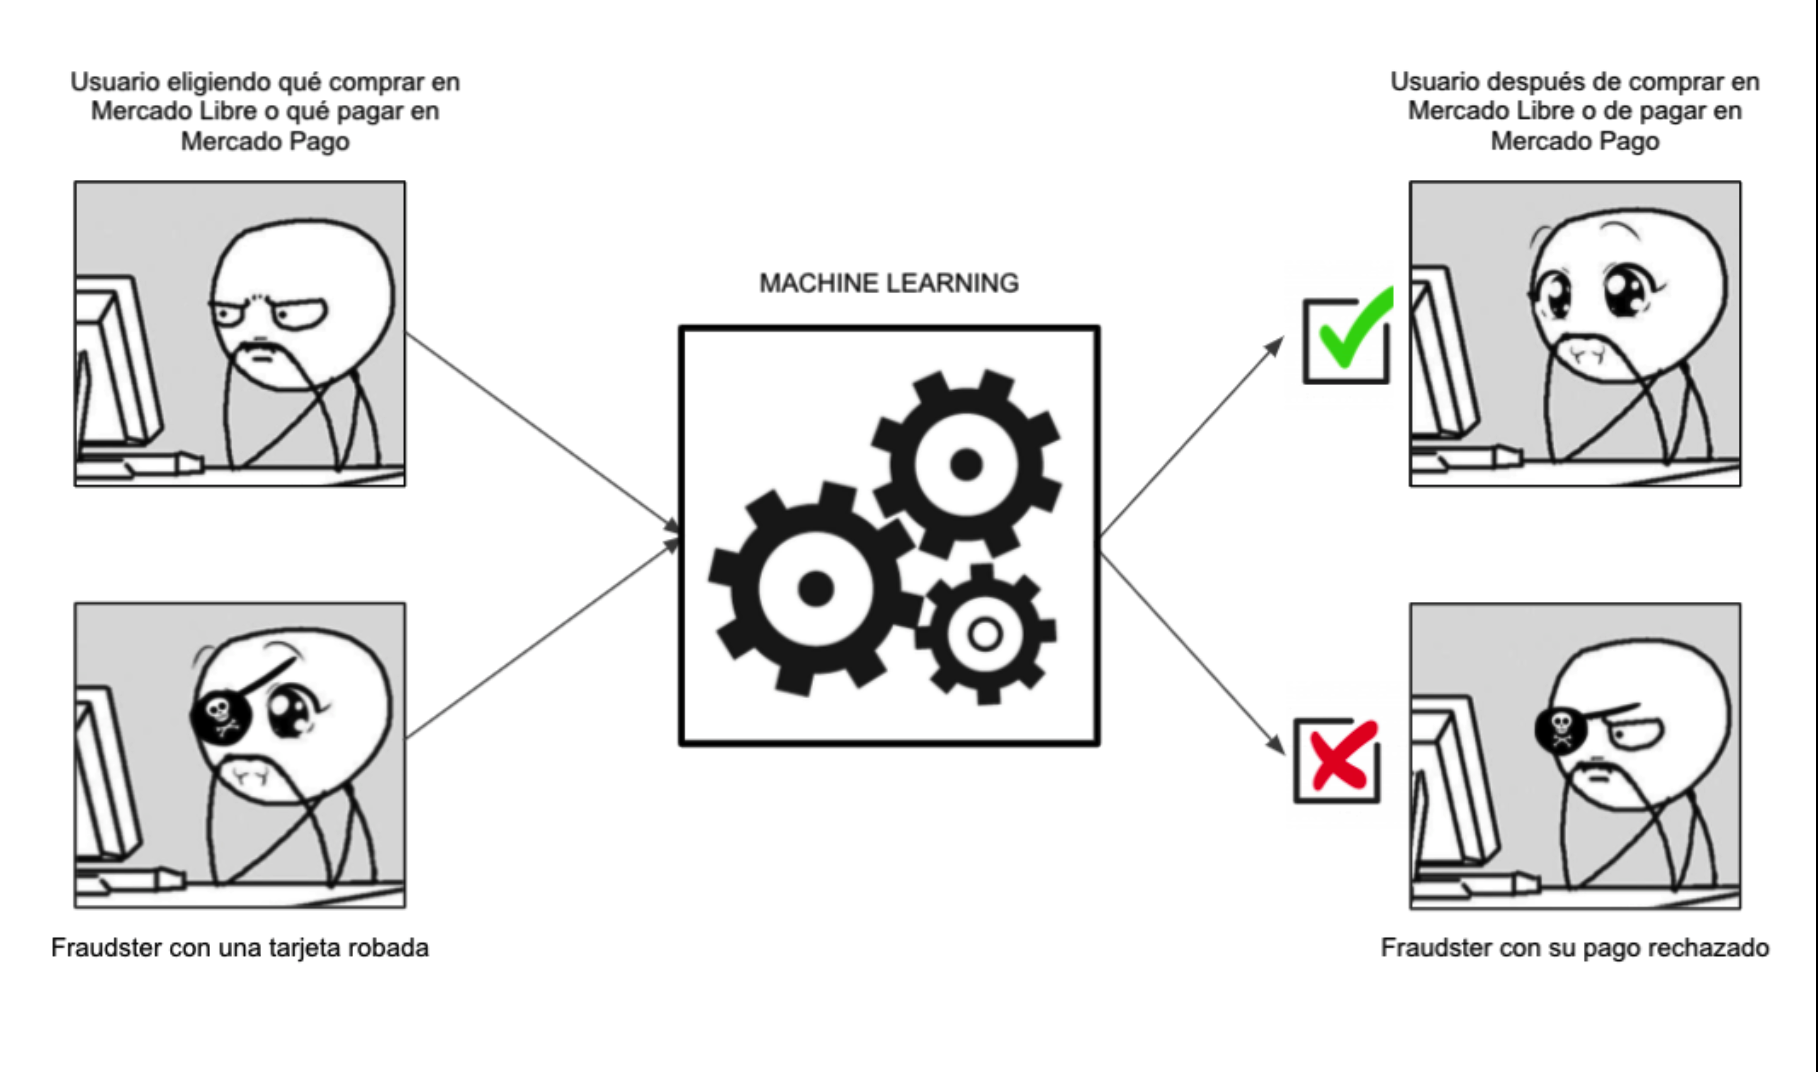
\includegraphics[width=.9\textwidth]{./Figuras/fraudster.png}}
\caption{Esquema del comportamiento esperado de los usuarios dentro de las plataformas de Meli.}
\label{fig:fraudster}
\end{figure}

El entrenamiento de modelos de machine learning para este tipo de aplicaciones conlleva una dificultad adicional: los datos de entrenamiento están fuertemente desbalanceados, es decir, la cantidad de pagos no fraudulentos es mucho mayor que la cantidad de pagos fraudulentos.

Para hacerle frente a este problema, lo que se propone hacer es entrenar un autoencoder, cuya arquitectura esquemática se muestra en la Figura \ref{fig:autoencoder}, sólo con pagos fraudulentos. De esta manera será posible enriquecer los registros de pagos que en el pasado fueron rechazados por ser riesgosos para poder tomarlos en cuenta en futuros entrenamientos. 

Por otro lado, el autoencoder presenta en su capa central o capa latente una representación reducida y codificada de la entrada. Es de esperarse que a partir de ella puedan visualizarse patrones de fraudes conocidos y, eventualmente, sacar conclusiones o indicios de patrones de fraudes sin conocer. El potencial de dicha representación puede verse en la Figura \ref{fig:latentRepresentation}.

\begin{figure}[H]
\centering
\frame{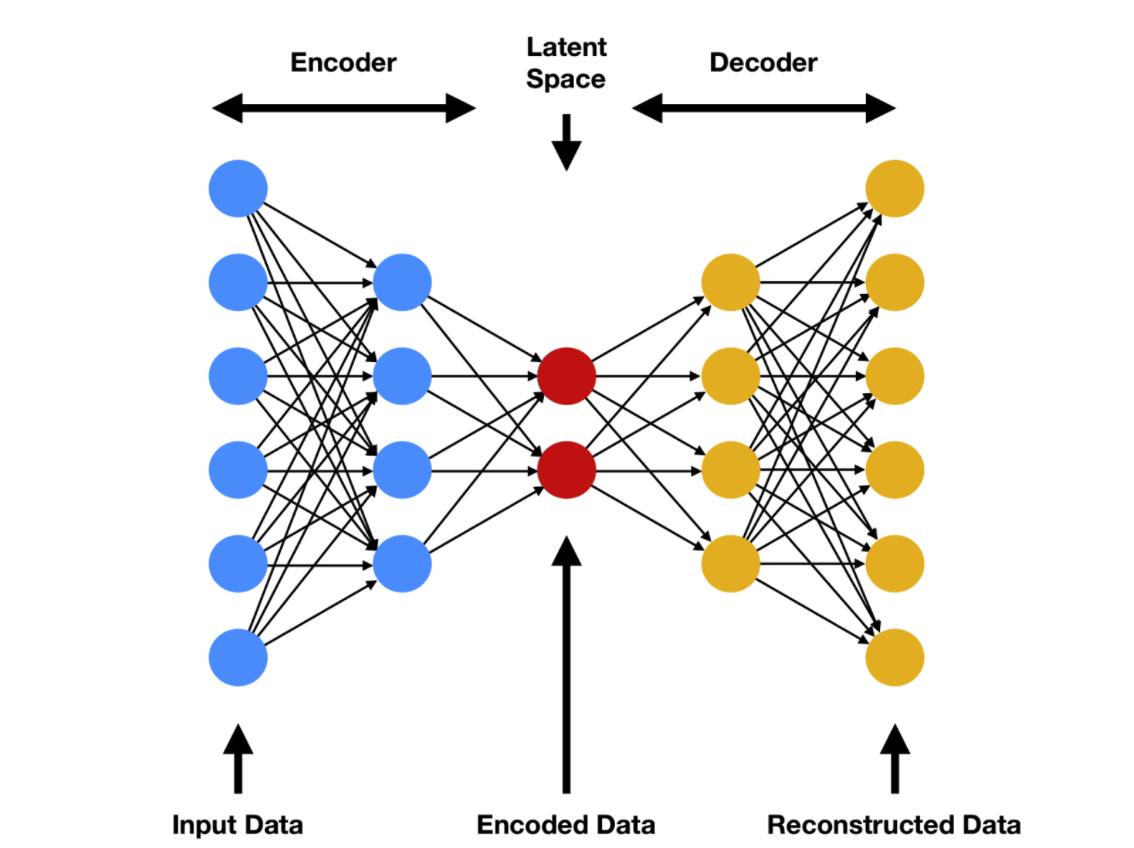
\includegraphics[width=.6\textwidth]{./Figuras/autoencoder.png}}
\caption{Arquitectura representativa de un autoencoder.}
\label{fig:autoencoder}
\end{figure}

\begin{figure}[H]
\centering
\subfloat[Descomposición de datos de entrada.]{\frame{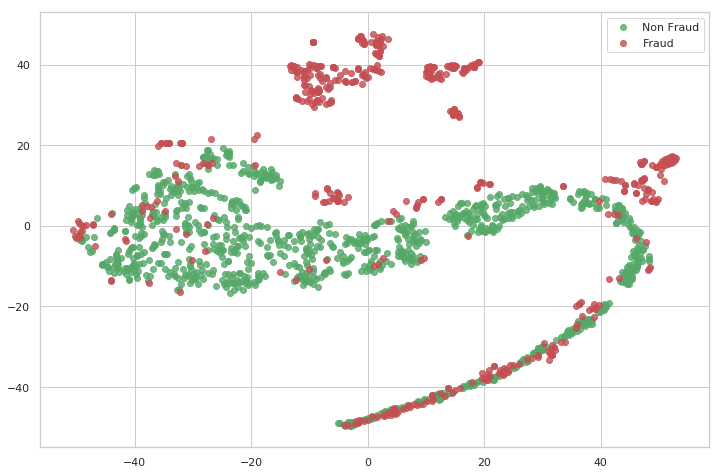
\includegraphics[width=0.47\textwidth]{./Figuras/actualRepr.png}}}
\hspace{0.05\textwidth}
\subfloat[Descomposición de datos latentes.]{\frame{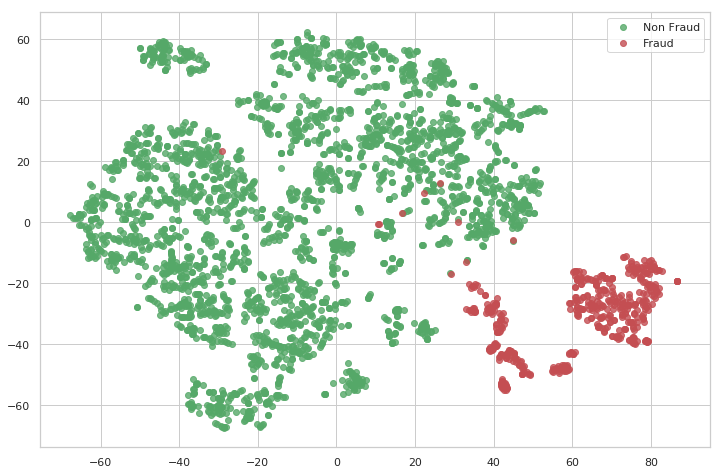
\includegraphics[width=0.47\textwidth]{./Figuras/latentRepr.png}}}
%\frame{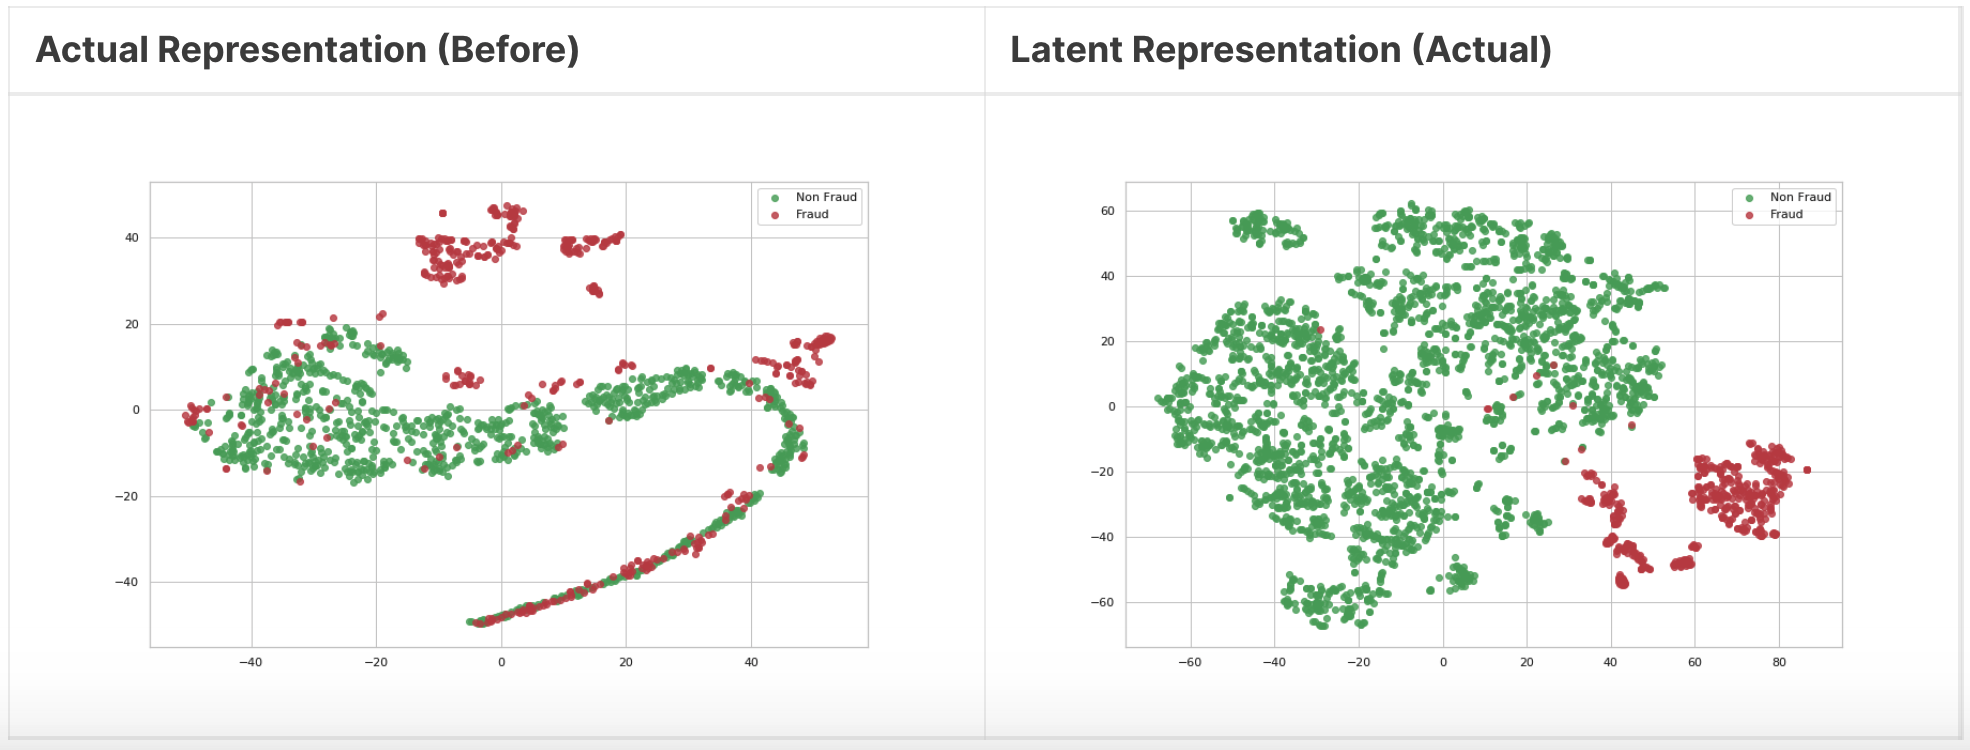
\includegraphics[width=\textwidth]{./Figuras/latentRepresentation.png}}
\caption{Imagen ilustrativa del artículo \emph{‘Semi Supervised Classification using AutoEnconders’} de Kaggle usando el método de descomposición T-SNE (\emph{t-Distributed Stochastic Neighbor Embedding}) aplicado a los datos.}
\label{fig:latentRepresentation}
\end{figure}

En la Figura \ref{fig:esquemaSistema} se observa un diagrama de bloques que ilustra cómo sería el funcionamiento del sistema en producción. En primer lugar, un usuario realizaría un pago en línea. Inmediatamente, el pago entra al sistema y se obtiene una representación vectorizada del mismo con los atributos de interés. Esta codificación del pago pasa por la red neuronal del motor de fraude y se obtiene una probabilidad de que el pago sea fraudulento (predicción). En función de la probabilidad de fraude y otros factores se decide si el pago se rechaza o se aprueba y se guardan todos los valores en una base de datos. En caso de que el pago sea rechazado, el mismo se envía al autoencoder de Fraude. Del autoencoder se obtendrá una puntuación de fraude asociada al pago rechazado que también se guardará en la base de datos. 

La puntuación de fraude será una medida de la capacidad de reconstrucción del autoencoder y  representará qué tan similar a un fraude real es el pago rechazado. Al momento de entrenar nuevos modelos de red o reentrenar modelos existentes, los pagos con alta puntuación podrán ser considerados en el dataset de entrenamiento. 

\begin{figure}[htpb]
\centering
\frame{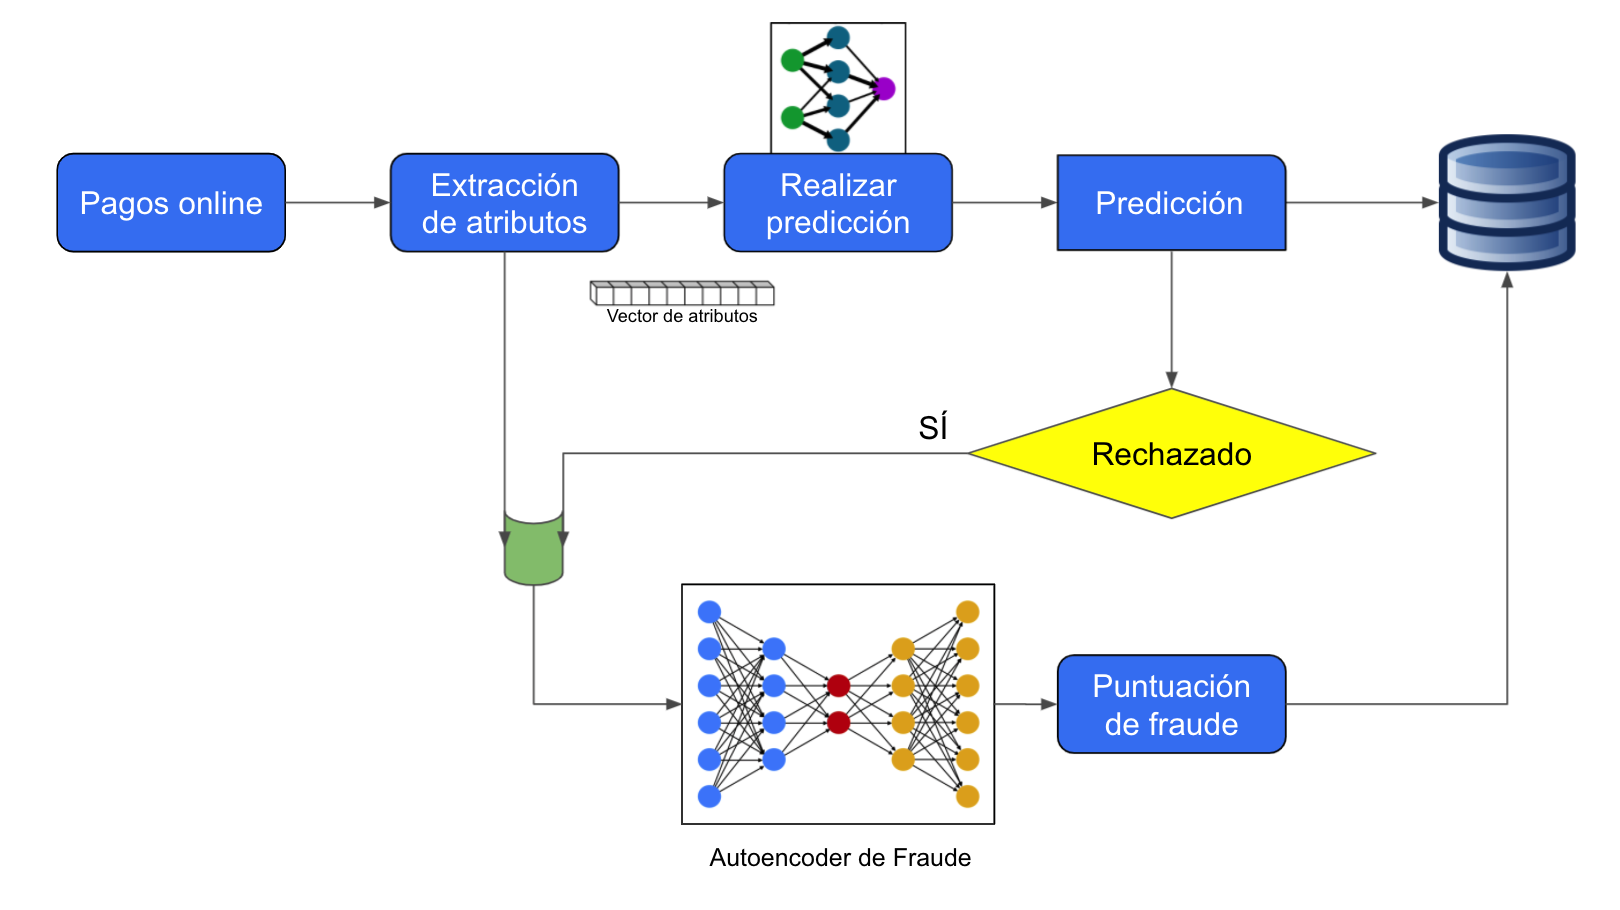
\includegraphics[width=\textwidth]{./Figuras/esquemaSistema.png}}
\caption{Diagrama de bloques del funcionamiento del sistema.}
\label{fig:esquemaSistema}
\end{figure}

\section{2. Identificación y análisis de los interesados}
\label{sec:interesados}

\begin{table}[ht]
\begin{tabularx}{\linewidth}{@{}|l|X|l|X|@{}}
\hline
\rowcolor[HTML]{C0C0C0} 
Rol           & Nombre y Apellido & Organización 	& Puesto 	\\ \hline
Responsable   & \authorname       & Mercado Libre   & ML Engineer \newline Alumno 	\\ \hline
Colaboradores & Ing. Paz Martin \newline 
    							Lcdo. Joaquín Loyola \newline 
    							Ing. Enrique Serdio    
    						& Mercado Libre  
    						& Sr. Data Scientist \newline 
    							Sr. Data Engineer \newline 
    							Sr. ML Engineer		\\ \hline
Orientador    & \supname	      & \pertesupname 	& Sr. ML Expert \newline Director Trabajo final \\ \hline
Usuario final & Desarrolladores de Machine Learning & Mercado Libre   & Data Scientists \newline ML Engineers       	\\ \hline
\end{tabularx}
\caption{Identificación de los interesados.}
\label{tab:interesados}
\end{table}

\begin{itemize}
	\item Responsable: \authorname, es la persona que desarrollará el proyecto.
	\item Colaboradores:
	\begin{itemize}
        \item{Paz Martín}: es líder y referente técnica del equipo de científicos de datos donde se desempeña el responsable. Validará la gestión del tiempo y será capaz de orientar en el desarrollo si el responsable lo requiriese. 
        \item{Joaquín Loyola}: es líder y referente técnico del equipo de ingeniería de datos. Su colaboración pasará por asistir al referente en cuestiones ligadas a los datos de entrenamiento, si fuese necesario.
        \item{Enrique Serdio}: es referente técnico del equipo de ML Ops. Su colaboración se centrará, si fuese necesario, en asistir al responsable en cuestiones ligadas a la infraestructura de los modelos de machine learning en la nube.
      \end{itemize}
	\item Orientador: Franco Arito es el director del presente proyecto y líder técnico de múltiples equipos de Mercado Libre. Su función será orientar al responsable a lo largo de la realización del proyecto.
	\item Desarrolladores de Machine Learning: son los usuarios finales que podrán hacer uso del sistema para enriquecer sus modelos.
\end{itemize}

\section{3. Propósito del proyecto}
\label{sec:proposito}
El propósito de este proyecto es poner en valor los pagos que son rechazados por el motor de fraude y que tienen potencial de ser utilizados en futuros entrenamientos de redes neuronales de manera tal de reducir el desbalance de los datasets de entrenamiento y validación. Además, se espera que la representación en la capa latente permita evaluar oportunidades para determinar perfiles de fraude. Con una representación como esta, los equipos de prevención tendrán a su disposición una herramienta que les permitirá ser más reactivos ante posibles ataques. 

\section{4. Alcance del proyecto}
\label{sec:alcance}
El proyecto comprenderá las siguientes etapas:
\begin{itemize}
\item Planificación de tareas.
\item Formación en TensorFlow.
\item Investigación de autoencoders aplicados a la prevención de fraude.
\item Selección y extracción del dataset para realizar prueba de concepto del modelo.
\item Análisis de datos del dataset.
\item Pruebas de arquitectura de red.
\item Visualización y análisis de datos de la capa latente utilizando el método de descomposición T-SNE.
\item Evaluación de distintas formas de hacer etiquetado (labeling).
\item Evaluación de la performance del sistema comparado con otras soluciones.
\item Evaluación del modelo con otros datasets.
\end{itemize}


El presente proyecto no incluye:
\begin{itemize}
\item Aplicación de algoritmos de clustering para los datos codificados a partir de la capa latente.
\item Despliegue del modelo y puesta en producción.
\end{itemize}


\section{5. Supuestos del proyecto}
\label{sec:supuestos}
Para el desarrollo del presente proyecto se supone que:
\begin{itemize}
	\item El responsable dispondrá de suficiente cantidad de tiempo para encarar los problemas que se presenten en el desarrollo del proyecto.
	\item El responsable tendrá a su disposición a su director y/o colaboradores cuando sea pertinente.
	\item TensorFlow es el framework de cálculo numérico que dispone de todas las herramientas necesarias para encarar este proyecto.
	\item El autoencoder entrenado solamente con pagos fraudulentos tendrá buen ratio de reconstrucción de datos a la hora de evaluar pagos rechazados por alto riesgo.
	\item La puntuación de fraude (asociada con la medida de reconstrucción de un pago) será un dato de tipo flotante, o bien, un dato de tipo categórico basado en ciertos valores de corte (thresholds). 
	\item Es posible aplicar el método de descomposición T-SNE a los datos codificados y, a partir de su representación en dos o tres dimensiones, se podrán realizar nuevos análisis, por ejemplo, la identificación de clusters de fraudes.
	\item Una vez que el autoencoder esté entrenado y validado con un set de pagos, su aplicación podrá generalizarse.
	\item El comportamiento de los usuarios que provocan el fraude no mutará mientras tiene lugar el desarrollo de este proyecto.
\end{itemize}

\section{6. Requerimientos}
\label{sec:requerimientos}

\begin{enumerate}
	\item Requerimientos de documentación
		\begin{enumerate}
			\item Toda documentación compartida debe mantenerse dentro de un acuerdo de confidencialidad.
			\item El trabajo debe ser continuamente documentado y se presentarán informes de avance una vez cada tres semanas al director.
			\item Los informes de avance pueden ser presentados como código correctamente documentado con los resultados correspondientes.
		\end{enumerate}
	\item Requerimientos de forma trabajo
		\begin{enumerate}
			\item Se utilizará una metodología de trabajo ágil e iterativa con mucha interacción entre el responsable, el director y los colaboradores.
		\end{enumerate}
	\item Requerimientos de lenguajes y frameworks
		\begin{enumerate}
			\item Los datos deberán ser consultados a base de datos relacionales. El lenguaje para estas transacciones debe ser SQL y debe ser lo más agnóstico posible intentando de no usar funciones que sean específicas de uno y otro proveedor.
			\item El framework utilizado debe ser Tensor Flow en su versión V2.0 o superior en Python.
			\item Todo análisis debe realizarse en código Python dentro de Jupyter labs y utilizando librerías standard  (numpy, pandas, matplotlib, seaborn, etcétera).
		\end{enumerate}
	\item Requerimientos de infraestructura
		\begin{enumerate}
			\item Las queries de extracción de datos deben ser compatibles con Amazon Redshift y/o Google BigQuery.
			\item Los datasets deben ser guardados en Amazon S3 o Google Cloud Storage como archivos con extensión \emph{.csv}.
			\item En caso de ser necesario un hardware específico de entrenamiento, deberán usarse los servicios de Google Cloud Platform (GCP).
		\end{enumerate}
	\item Requerimientos funcionales
		\begin{enumerate}
			\item La extracción de datos no puede demorar más de 24 hs.
			\item El modelo entrenado debe tener una precisión de al menos 85\%.
			\item El modelo debe ser entrenado con al menos diez mil registros.
			\item El entrenamiento del modelo no puede demorar más de 24 hs.
			\item El tipo de dato que represente la puntuación de fraude debe ser categórico o flotante.
			\item Las representaciones resultantes de la descomposición deben poder visualizarse en dos o tres dimensiones.
		\end{enumerate}
	\item Requerimientos de testing y evaluación
		\begin{enumerate}
			\item La efectividad de la puntuación de fraude debe ser evaluada contra una marca dada por una heurística conocida y la efectividad de la puntuación debe ser mejor que la efectividad de la marca.
		\end{enumerate}
\end{enumerate}

\section{7. Historias de usuarios (\textit{Product backlog})}
\label{sec:backlog}
La medida del trabajo a efectuar para cumplir con cada una de las historias de usuarios estará dada por \emph{story points}. Para ponderar los esfuerzos se utilizará la serie de Fibonacci con valores: 0, 1, 2, 3, 5, 8, 13, 21, 34, 55, 89, etc. Cuando el esfuerzo se considere alto los \emph{story points} tomarán valores entre 0 y 3 inclusive. Cuando se considere medio, entre 5 y 13 inclusive. Cuando el esfuerzo se considere alto el valor de los \emph{story points} será igual o mayor a 21.

\begin{itemize}
\item Como analista y desarrollador quiero una métrica de fraude para reutilizar pagos rechazados por alto riesgo en futuros entrenamientos y futuros análisis. 

Dificultad: Alta (34) -- Complejidad: Alta (34)  -- Incertidumbre: Alta (34)

Story Points: 34 + 34 + 34 = 102 $\rightarrow$ 89

\item Como cliente quiero tener un modelo de red realizado con tecnologías standards y \emph{open source} para poder mantenerlo a futuro con el menor esfuerzo posible.

Dificultad: Media (8) -- Complejidad: Media (8) -- Incertidumbre: Baja (1)

Story Points: 8 + 8 + 1 = 17 $\rightarrow$ 21

\item Como analista de datos quiero tener una representación simplificada del fraude para entender posibles ataques y ser reactivo en consecuencia.

Dificultad: Alta (21)  -- Complejidad: Alta (21) -- Incertidumbre: Alta (21)

Story Points: 21 + 21 + 21 = 63 $\rightarrow$  55

\item Como cliente quiero tener las bases de un modelo de red preciso para servirlo en producción adaptándose a flujos preexistentes.

Dificultad: Media (8) -- Complejidad: Media (8) -- Incertidumbre: Alta (21)

Story Points: 8 + 8 + 21 = 37 $\rightarrow$ 34

\item Como cliente quiero recibir la documentación del trabajo realizado para que pueda servir como base de futuros desarrollos de la empresa.

Dificultad: Media (13) -- Complejidad: Baja (2) -- Incertidumbre: Baja (1)

Story Points: 13 + 2 + 1 = 16 $\rightarrow$ 13

\item Como cliente quiero tener una presentación resumida del trabajo para mostrar sus resultados y su potencial potencial a todos los interesados.

Dificultad: Baja (3) -- Complejidad: Baja (2) -- Incertidumbre: Baja (2)

Story Points: 3 + 2 + 2 = 7 $\rightarrow$ 8


\end{itemize}

\section{8. Entregables principales del proyecto}
\label{sec:entregables}

Los entregables del proyecto que conservará la empresa donde trabaja el responsable y el director son:

\begin{itemize}
 \item Informe final.
 \item Presentación final.
 \item Datasets utilizados.
 \item Queries de extracción documentadas.
 \item Jupyter labs de análisis documentados.
 \item Informe de avance.
\end{itemize}

Además, se entregará a los docentes responsables de la Carrera de Especialización en Inteligencia Artificial de la UBA informe de avance y el informe final del proyecto con firma previa de los documentos de confidencialidad.

\section{9. Desglose del trabajo en tareas}
\label{sec:wbs}


\begin{enumerate}
\item Planificación. (60 hs)
	\begin{enumerate}
		\item Estudio de necesidades. (9 hs)
		\item Análisis de factibilidad. (3 hs)
		\item Definición de requerimientos. (9 hs)
		\item Confección de documento de planificación. (39 hs)
	\end{enumerate}
\item Investigación y capacitación. (114 hs)
	\begin{enumerate}
		\item Estudio de distintos tipos de autoencoders. (9 hs)
		\item Estudio de autoencoders aplicados a la prevención de fraude. (3 hs)
		\item Capacitación en Tensor Flow 2. (15 hs)
		\item Capacitación en \emph{feature preprocessing} y \emph{feature engineering}. (24 hs)
		\item Capacitación en \emph{feature selection}. (15 hs)
		\item Capacitación en SQL aplicado a Amazon Redshift y Google BigQuery. (9 hs)
		\item Capacitación en \emph{Machine Learning pipelines} en GCP. (15 hs)
		\item Estudio de algoritmo T-SNE. (9 hs)
		\item Elaboración de códigos de ejemplos básicos. (15 hs)
	\end{enumerate}
\item Confección dataset de prueba. (45 hs)
	\begin{enumerate}
		\item Exploración y elección tablas. (9 hs)
		\item Análisis de completitud de datos. (9 hs)
		\item Confección de query de extracción. (9 hs)
		\item Extracción de datos. (3 hs)
		\item Selección de features. (15 hs)
	\end{enumerate}
\item Entrenamiento. (78 hs)
	\begin{enumerate}
		\item Aplicación de \emph{feature preprocessing}. (15 hs)
		\item Prueba de distintas arquitecturas de red con distintas configuraciones. (39 hs)
		\item Evaluación y ajuste del modelo. (24 hs)
	\end{enumerate}
\item Pruebas de validación. (63 hs)
	\begin{enumerate}
		\item Evaluación de distintas estrategias de \emph{labeling}. (39 hs)
		\item Comparación de resultados en función de heurísitcas conocidas. (24 hs)
	\end{enumerate}
\item Representación reducida. (63 hs)
	\begin{enumerate}
 		\item Visualización de datos de la capa de entrada utilizando el método de descomposición T-SNE. (15 hs)
 		\item Visualización de datos de la capa latente utilizando el método de descomposición T-SNE. (15 hs)
 		\item Visualización segmentada de los datos en función de features de interés del modelo. (33 hs)
 	\end{enumerate}
\item Generalización. (87 hs)
 	\begin{enumerate}
 		\item Extracción de datos correspondientes a otro flujo de datos. (24 hs)
 		\item Análisis de completitud de datos. (15 hs)
 		\item Comparación y análisis de resultados. (24 hs)
 		\item Ajustes finales. (24 hs)
 	\end{enumerate}
\item Documentación y presentación final. (90 hs)
 	\begin{enumerate}
 		\item Elaborar informe de avance proyecto. (40 hs)
 		\item Elaborar informe final del proyecto. (40 hs)
 		\item Preparación de presentación final. (30 hs)
 	\end{enumerate}
\end{enumerate}

Cantidad total de horas: (630 hs)

\section{10. Diagrama de Activity On Node}
\label{sec:AoN}

En la Figura \ref{fig:aon} se muestra el diagrama de \emph{Activity on Node} del proyecto. Las flechas resaltadas en negro ilustran el camino crítico del proyecto. También se puede ver que los hitos marcan el fin de las distintas fases del proyecto, las cuales, a su vez, están representadas en distintos colores. 

La primera fase está comprendida por tareas previas al desarrollo en código del proyecto. En esta fase se considera planificación y capacitación.

La segunda fase involucra todo el \emph{machine learning pipeline} necesario para evaluar entrenar un modelo y dejarlo preparado para en un futuro servirlo en producción.

La tercera fase toma como punto de partida un modelo de calidad ya entrenado e intenta agregarle valor al mismo mediante la generalización de resultados y la representación reducida de los pagos para intentar obtener otras posibles conclusiones adicionales relacionadas con potenciales perfiles de fraude.

Finalmente, la última fase, involucra toda la realización de toda la documentación del trabajo realizado.

\begin{figure}[htpb]
\centering 
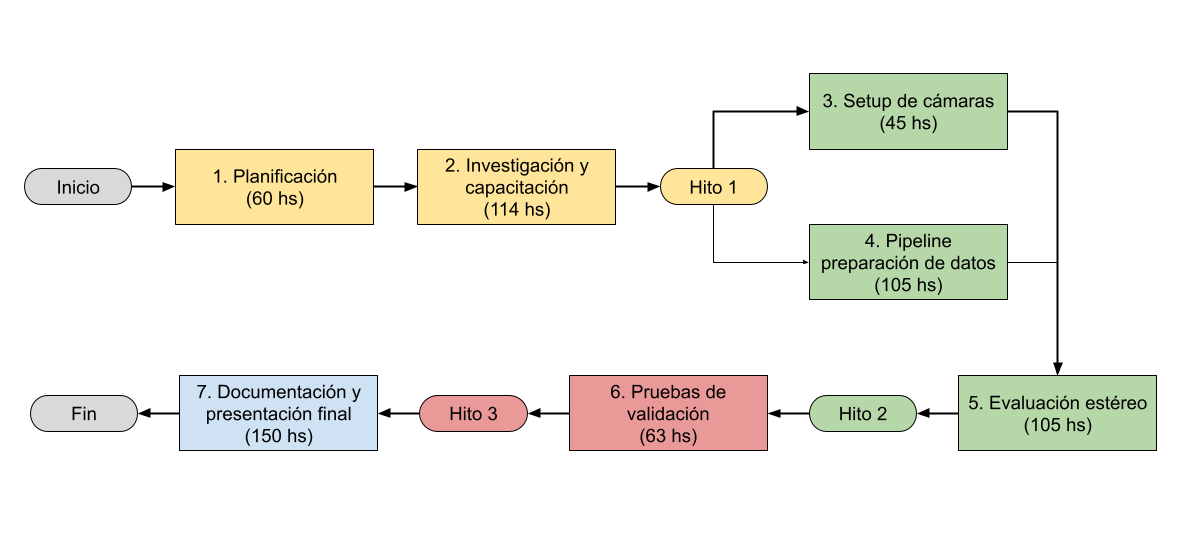
\includegraphics[width=\textwidth]{./Figuras/aon.png}
\caption{Diagrama en \textit{Activity on Node.}}
\label{fig:aon}
\end{figure}

\section{11. Diagrama de Gantt}
\label{sec:gantt}

A continuación se muestra el diagrama de Gant del presente proyecto. Se consideró la jornada laboral de 3 horas de trabajo desde la fecha de inicio del curso hasta finales de abril del próximo año.
En la figura \ref{fig:ganttReducido} y \ref{fig:ganttCompleto} se muestra el diagrama de Gantt de forma compacta y de forma desglosada respectivamente, tal como se enumeró en la sección 9.

\begin{figure}[htpb]
\centering 
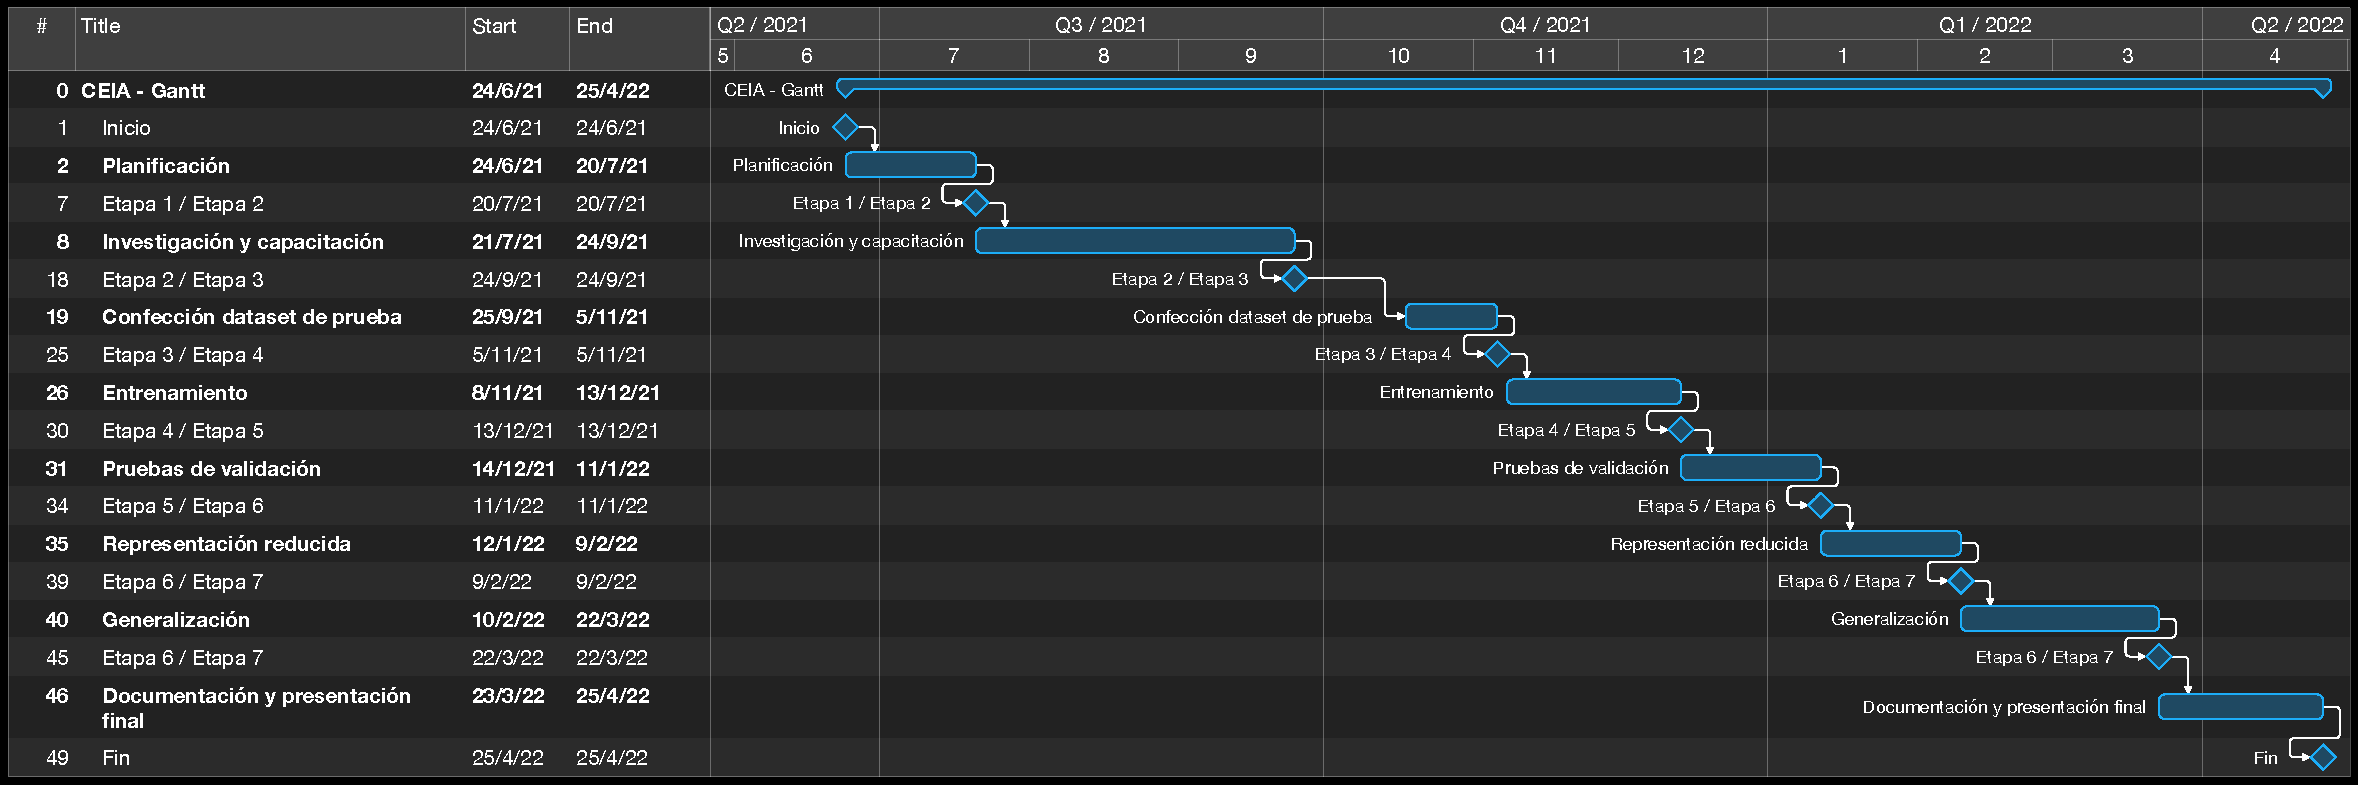
\includegraphics[width=\textwidth]{./Figuras/ganttReducido.pdf}
\caption{Diagrama de Gantt reducido.}
\label{fig:ganttReducido}
\end{figure}

\begin{figure}[htpb]
\centering 
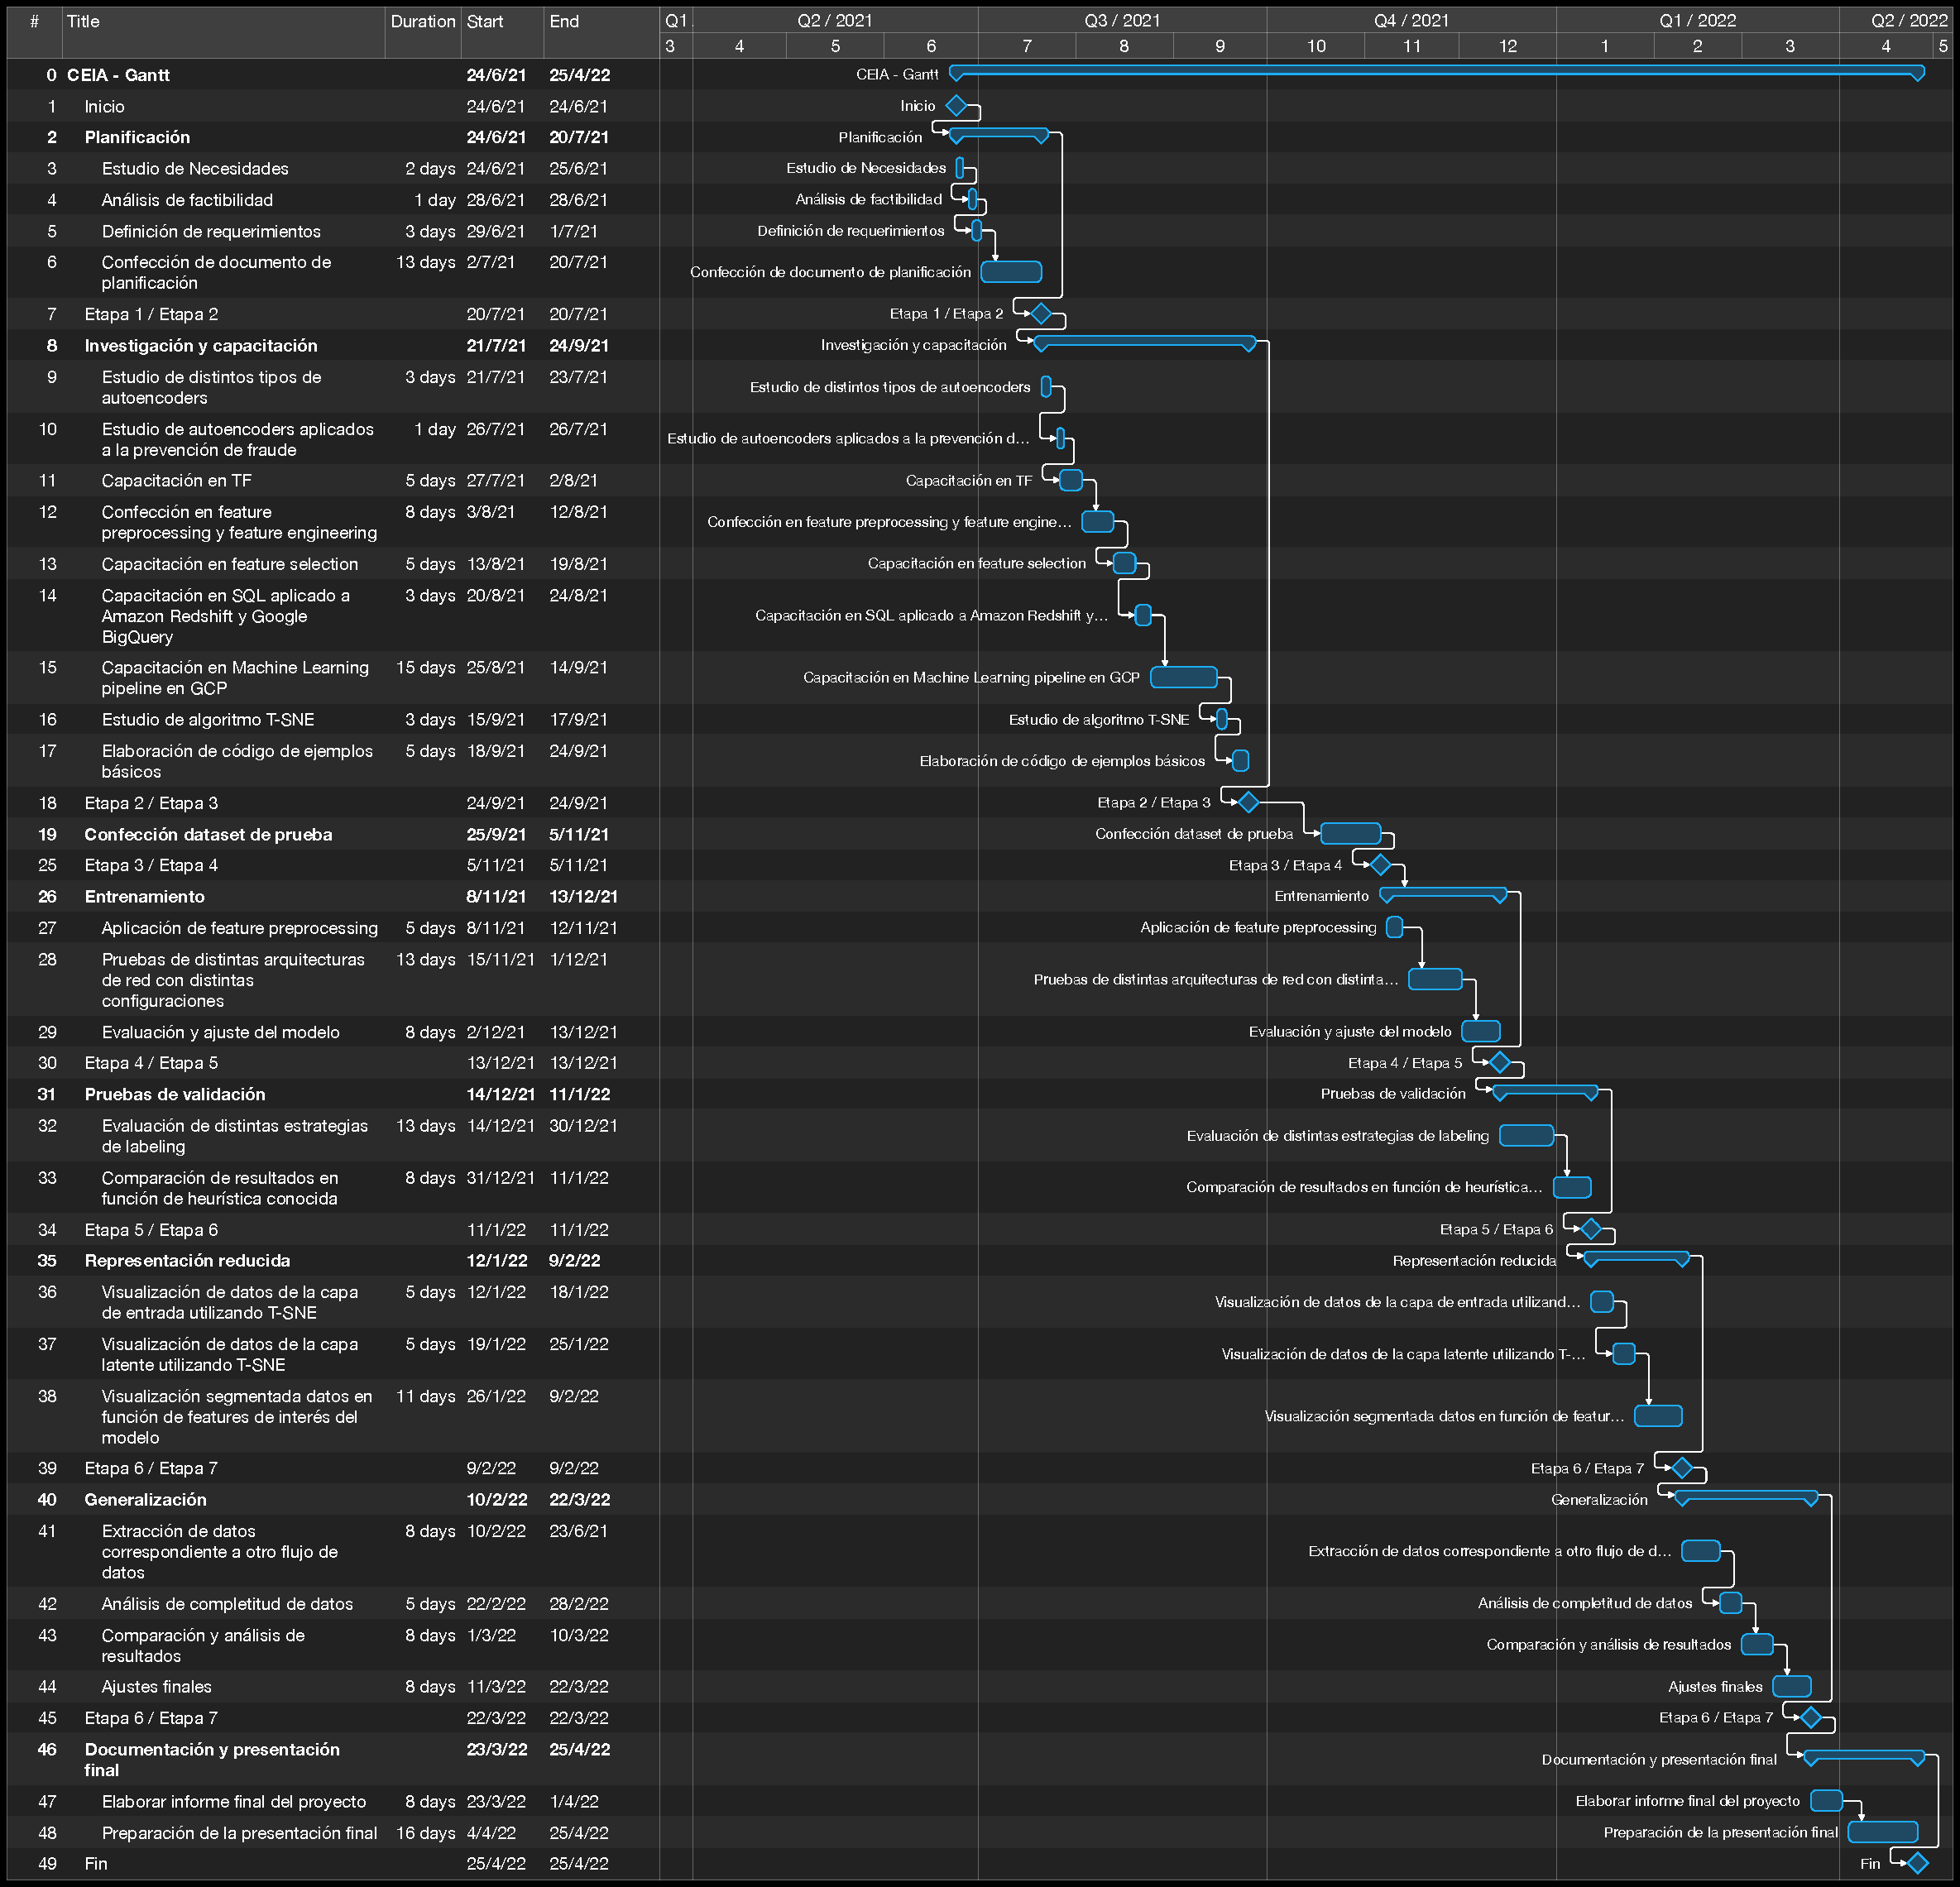
\includegraphics[width=\textwidth,  height=0.9\textheight]{./Figuras/ganttCompleto.pdf}
\caption{Diagrama de Gantt desglosado en tareas.}
\label{fig:ganttCompleto}
\end{figure}

\section{12. Presupuesto detallado del proyecto}
\label{sec:presupuesto}

En esta sección se detallan los gastos del proyecto. Las unidades del valor unitario están dadas en dólares estadounidenses.

Las cantidades del uso de los servicios son estimadas. En el caso de Amazon Redshift y Google BigQuery se ha considerado el gasto mensual fijo del uso del servicio que paga la empresa. En el caso de Amazon Redshift se ha estimado que se almacenará 1 Terabyte de información durante 10 meses. Finalmente, para el caso de entrenamientos, se ha considerado que los entrenamientos de los experimentos durarán 50 horas y tendrán lugar durante un mes.

\begin{table}[htpb]
\centering
\begin{tabularx}{\linewidth}{@{}|X|c|r|r|@{}}
\hline
\rowcolor[HTML]{C0C0C0} 
\multicolumn{4}{|c|}{\cellcolor[HTML]{C0C0C0}COSTOS DIRECTOS} \\ \hline
\rowcolor[HTML]{C0C0C0} 
Descripción &
  \multicolumn{1}{c|}{\cellcolor[HTML]{C0C0C0}Cantidad} &
  \multicolumn{1}{c|}{\cellcolor[HTML]{C0C0C0}Valor unitario} &
  \multicolumn{1}{c|}{\cellcolor[HTML]{C0C0C0}Valor total [USD]} \\ \hline
 	Mano de obra & 
  	\multicolumn{1}{c|}{600 horas} &
  	\multicolumn{1}{c|}{10 USD/hora} &
  	\multicolumn{1}{c|}{6300} \\ \hline
 	Google BigQuery &
  	\multicolumn{1}{c|}{1 mes} &
  	\multicolumn{1}{c|}{1700 USD/mes} &
  	\multicolumn{1}{c|}{1700} \\ \hline
 	Amazon Redshift &
  	\multicolumn{1}{c|}{1 mes} &
  	\multicolumn{1}{c|}{1380 USD/mes} &
  	\multicolumn{1}{c|}{1380} \\ \hline
 	Amazon S3 &
  	\multicolumn{1}{c|}{1 TB 10 meses} &
  	\multicolumn{1}{c|}{0.0.23 USD/GB/mes} &
  	\multicolumn{1}{c|}{235.52} \\ \hline
 	Google AI Platform &
  	\multicolumn{1}{c|}{1 mes} &
  	\multicolumn{1}{c|}{61.05 USD/mes} &
  	\multicolumn{1}{c|}{61.05} \\ \hline
\multicolumn{3}{|c|}{SUBTOTAL} &
  \multicolumn{1}{c|}{9676.57} \\ \hline
\rowcolor[HTML]{C0C0C0} 
\multicolumn{4}{|c|}{\cellcolor[HTML]{C0C0C0}COSTOS INDIRECTOS} \\ \hline
\rowcolor[HTML]{C0C0C0} 
Descripción &
  \multicolumn{1}{c|}{\cellcolor[HTML]{C0C0C0}Cantidad} &
  \multicolumn{1}{c|}{\cellcolor[HTML]{C0C0C0}Valor unitario} &
  \multicolumn{1}{c|}{\cellcolor[HTML]{C0C0C0}Valor total [USD]} \\ \hline
	30\% del costo directo & 
  	\multicolumn{1}{c|}{-} &
  	\multicolumn{1}{c|}{-} &
  	\multicolumn{1}{c|}{2812.97} \\ \hline
\multicolumn{3}{|c|}{SUBTOTAL} &
  \multicolumn{1}{c|}{2902.97} \\ \hline
\rowcolor[HTML]{C0C0C0}
\multicolumn{3}{|c|}{TOTAL} &
   \multicolumn{1}{c|}{12579.54} \\ \hline
\end{tabularx}%
\end{table}


\section{13. Gestión de riesgos}
\label{sec:riesgos}

a) Identificación de los riesgos del proyecto:

Riesgo 1: falta de disponibilidad de los colaboradores.
\begin{itemize}
	\item Severidad (3): ante la ausencia de alguno de los colaboradores, se hará más largo el desarrollo en los cuellos de botella del proyecto.
	\item Probabilidad de ocurrencia (7): hay mucha rotación de empleados en la empresa y colaborador podría dejarla durante el transcurso del proyecto. 
\end{itemize}

Riesgo 2: falta de tiempo del responsable.
\begin{itemize}
	\item Severidad (5): se atrasarían las tareas, no se cumpliría con la planificación y, en el peor de los casos, no se lograría completar el proyecto para la fecha de presentación establecida.
	\item Probabilidad de ocurrencia (4): en la empresa donde trabaja el responsable surgen contingencias que son prioritarias. 
\end{itemize}   

Riesgo 3: no llegar a un 85\% de precisión en el entrenamiento. 
\begin{itemize}
	\item Severidad (8): no se contaría con una red entrenada de calidad y los resultados de la misma no serían tan fiables.
	\item Probabilidad de ocurrencia (3): puede ocurrir que los datos seleccionados para el entrenamiento no sean lo suficientemente representativos. 
\end{itemize}

Riesgo 4: comportamiento inesperado del modelo a la hora de predecir. 
\begin{itemize}
	\item Severidad (9): si el modelo tiene un buen ratio de reconstrucción para pagos fraudulentos y resulta que también tiene un buen ratio de reconstrucción para los pagos no fraudulentos no se cumpliría la hipótesis planteada en este trabajo.
	\item Probabilidad de ocurrencia (3): es posible que la red no aprenda los patrones que permitan distinguir un pago fraudulento de un pago no fraudulento.
\end{itemize}

Riesgo 5: efectividad de puntuación de fraude menor a marca de heurística.
\begin{itemize}
	\item Severidad (9): si esto sucede no se cumpliría con la motivación del trabajo.
	\item Probabilidad de ocurrencia (4): puede que la red neuronal no aprenda patrones que permitan separar pagos fraudulentos de no fraudulentos y, por ello, la puntuación de fraude puede no ser eficiente. También puede ocurrir que el modelo se comporte de la manera esperada pero que aún así no llegue a superar la eficiencia de la marca heurística. 
\end{itemize}

Riesgo 6: no llegar a distinguir patrones en la representación reducida.
\begin{itemize}
	\item Severidad (3): no es tan grave que no se puedan distinguir patrones de fraude dentro del set de datos. No es la motivación principal de este proyecto.
	\item Probabilidad de ocurrencia (5): es una hipótesis donde se tiene gran incertidumbre.
\end{itemize}

b) Tabla de gestión de riesgos:      (El RPN se calcula como RPN=SxO)

\begin{table}[htpb]
\centering
\begin{tabularx}{\linewidth}{@{}|X|c|c|c|c|c|c|@{}}
\hline
\rowcolor[HTML]{C0C0C0} 
Riesgo & S & O & RPN & S* & O* & RPN* \\ \hline
		Falta de disponibilidad de los colaboradores & 3  & 7  & 21 & - & - &  21 \\ \hline
       Falta de tiempo del responsable & 5  & 4  & 20 & - & - & 20 \\ \hline
       No llegar a un 85\% de precisión en el entrenamiento & 8  & 3  & 24 & 6 & 2 & 12     \\ \hline
       Comportamiento inesperado del modelo a la hora de predecir & 9  & 3  & 27 &  8  &  2  &  16    \\ \hline
       Efectividad de puntuación de fraude menor a marca de heurística & 9 & 4 & 36 & 8 & 2 & 16     \\ \hline
      No llegar a distinguir patrones en la representación reducida & 3 &  5 & 15 & -  & -   & 15  \\ \hline
\end{tabularx}
\end{table}

Criterio adoptado: se tomarán medidas de mitigación en los riesgos cuyos números de RPN sean mayores a 21.

Nota: los valores marcados con (*) en la tabla corresponden luego de haber aplicado la mitigación.


c) Plan de mitigación de los riesgos que originalmente excedían el RPN máximo establecido:
 
Riesgo 3: no llegar a un 85\% de precisión en el entrenamiento.
\begin{itemize}
	\item Plan de mitigación: en primer lugar se atacará la red. Se seguirán probando distintas arquitecturas y distintos hiperparámetros. Si eso no da resultado se buscarán más datos y se hará una nueva extracción con más registros y más \emph{features}.
	\item Severidad (6): cada uno de los planes de mitigación conlleva un tiempo adicional no menor por lo que la planificación del proyecto podría verse atrasada.
	\item Probabilidad de ocurrencia (2): haciendo todos los ajustes posibles debería alcanzarse la precisión deseada.
\end{itemize}

Riesgo 4: comportamiento inesperado del modelo a la hora de predecir. 
\begin{itemize}
	\item Plan de mitigación: se invertirá el paradigma del trabajo. El objetivo se planteó de manera tal de entrenar un autoencoder con pagos fraudulentos para estimar, dentro de los pagos rechazados, cuántos estuvieron bien rechazados. La mitigación consistirá en entrenar el autoencoder con pagos no fraudulentos para medir, dentro de los rechazados, cuántos estuvieron mal rechazados. Esto puede hacerse porque la cantidad de pagos no fraudulentos es mucho mayor que la cantidad de pagos fraudulentos y, además, la dinámica del comportamiento del usuario no fraudulento es mucho menor que la dinámica de comportamiento del usuario no fraudulento.
	\item Severidad (8): tomar el enfoque del plan de mitigación seguramente daría buenos resultados pero se perdería mucho tiempo en nuevas extracciones y pre procesamiento de datos. Además la representación reducida de dichos pagos no tendría mucho valor.
	\item Probabilidad de ocurrencia (2): es muy improbable que con la gran cantidad de datos disponibles no se pueda ajustar la red para que pueda predecir correctamente.
\end{itemize}

Riesgo 5: efectividad de puntuación de fraude menor a marca de heurística.
\begin{itemize}
	\item Plan de mitigación: se convocará al director o a alguno de los colaboradores para que participen activamente en la mejora.
	\item Severidad (8): poner mucho recurso humano a mitigar el problema seguramente impactará en grandes retrasos en la planificación.
	\item Probabilidad de ocurrencia (2): sería raro que surgiese este problema sin que se hubiese advertido y eventualmente, mitigado, en pasos anteriores.
\end{itemize}




\section{14. Gestión de la calidad}
\label{sec:calidad}

\begin{itemize} 

\item Req 1.1: toda documentación compartida debe mantenerse dentro de un acuerdo de confidencialidad.
\begin{itemize}
	\item Verificación: se firmará acuerdo de confidencialidad entre las partes. 
	\item Validación: revisión y conformidad por parte del director.
\end{itemize}

\item Req 1.2: el trabajo debe ser continuamente documentado y se presentarán informes de avance una vez cada tres semanas al director.
\begin{itemize}
	\item Verificación: se controlará que cada avance tenga la documentación necesaria de manera que alguno de los colaboradores pueda entender el avance sin entrar en detalles de implementación. 
	\item Validación: revisión y conformidad por parte del director.
\end{itemize}

\item Req 1.3: los informes de avance pueden ser presentados como código correctamente documentado con los resultados correspondientes.
\begin{itemize}
	\item Verificación: se controlará que cada avance tenga la documentación necesaria de manera que alguno de los colaboradores pueda entender el avance sin entrar en detalles de implementación. 
	\item Validación: revisión y conformidad por parte del director.
\end{itemize}

\item Req 2.1: se utilizará una metodología de trabajo  ágil e iterativa con mucha interacción entre el responsable, el director y los colaboradores.
\begin{itemize}
	\item Verificación: se realizarán todas las ceremonias que correspondan y se comentarán los problemas y/o avances en las \emph{dailys} que correspondan.
	\item Validación: N/A (requerimiento interno).
\end{itemize}

\item Req 3.1: los datos deberán ser consultados a base de datos relacionales. El lenguaje para estas transacciones debe ser SQL y debe ser lo más agnóstico posible (intentar no usar funciones que sean específicas de uno y otro proveedor).
\begin{itemize}
	\item Verificación: se probarán las queries en distintos proveedores para asegurarse de que corra en todos.
	\item Validación: N/A (requerimiento interno).
\end{itemize}

\item Req 3.2: el framework utilizado debe ser Tensor Flow en su versión V2.0 o superior en Python.
\begin{itemize}
	\item Verificación: al comienzo de cada sesión de trabajo se utilizará el comando \emph{pip show tesorflow} para verificar la versión utilizada.
	\item Validación: N/A (requerimiento interno).
\end{itemize}

\item Req 3.3: todo análisis debe realizarse en código Python dentro de Jupyter labs y utilizando librerías standard (numpy, pandas, matplotlib, seaborn, etcétera).
\begin{itemize}
	\item Verificación: todo el código escrito se volcará en una máquina virtual provista de un Jupyter Lab con todas las librerías standard pre instaladas. 
	\item Validación: N/A (requerimiento interno).
\end{itemize}

\item Req 4.1: las queries de extracción de datos deben ser compatibles con Amazon Redshift y/o Google BigQuery.
\begin{itemize}
	\item Verificación: se probarán las queries en uno y otro proveedor con registros limitados. 
	\item Validación: N/A (requerimiento interno).
\end{itemize}

\item Req 4.2: los datasets deben ser guardados en Amazon S3 o Google Cloud Storage como archivos con extensión .csv.
\begin{itemize}
	\item Verificación: se podrán consultar cada uno de los archivos en el bucket que corresponda.
	\item Validación: N/A (requerimiento interno).
\end{itemize}

\item Req 4.3: en caso de ser necesario un hardware específico de entrenamiento, deberán usarse los servicios de Google Cloud Platform (GCP).
\begin{itemize}
	\item Verificación: se harán ensayos de entrenamiento en una máquina local y en máquinas remotas que a lo sumo estarán provistas de GPU. En caso de no cumplir con los requerimientos de entrenamiento, se solicitará usar una máquina virtual provista de TPU.
	\item Validación: revisión y conformidad por parte del director.
\end{itemize}

\item Req 5.1: la extracción de datos no puede demorar más de 24 hs.
\begin{itemize}
	\item Verificación: se harán extracciones de prueba con datos reducidos. En función de los resultados se hará una estimación de cuánto puede llegar a demorar una extracción de calidad para cumplir con el requerimiento.
	\item Validación: la extracción se configurará para parar por \emph{timeout} a las 24 hs.
\end{itemize}

\item Req 5.2: el modelo entrenado debe tener una precisión de al menos 85\%.
\begin{itemize}
	\item Verificación: se tendrán los resultados en entrenamiento en las tablas de métricas de Tensor Flow para consultar y verificar.
	\item Validación: cuando el sistema se ponga en producción se monitoreará para validar la métrica antes mencionada.
\end{itemize}

\item Req 5.3: el modelo debe ser entrenado con al menos diez mil registros.
\begin{itemize}
	\item Verificación: se tendrá un contador de registros presentes en la extracción resultante.
	\item Validación: N/A (requerimiento interno).
\end{itemize}

\item Req 5.4: el entrenamiento del modelo no puede demorar más de 24 hs.
\begin{itemize}
	\item Verificación: se harán entrenamientos de prueba con modelos sencillos para ver cuánto dura un entrenamiento de este estilo. En función de los resultados se hará una estimación de cuánto puede llegar a complejizarse el modelo para cumplir con el requerimiento.
	\item Validación: el entrenamiento se configurará para parar por \emph{timeout} a las 24 hs.
\end{itemize}

\item Req 5.5: el tipo de dato que represente la puntuación de fraude debe ser categórico o flotante.
\begin{itemize}
	\item Verificación: se realizarán distintas pruebas analizando la dispersión de los resultados obtenidos para saber si es posible simplificar el grado de reconstrucción a una variable categórica binaria.
	\item Validación: revisión y conformidad por parte del director.
\end{itemize}

\item Req 5.6: las representaciones resultantes de la descomposición deben poder visualizarse en dos o tres dimensiones.
\begin{itemize}
	\item Verificación: una vez que el modelo del autoencoder esté entrenado el modelo de la red se seccionará de forma tal de tener como capa de salida la capa latente. Cada uno de los pagos que forman parte de los set de entrenamiento, validación y test pasarán por esta red de codificación. Una vez que se tienen los datos codificados o latentes, se le aplicará el algoritmo T-SNE y los resultados se graficarán usando matplotlib. 
	\item Validación: N/A (requerimiento interno).
\end{itemize}

\item Req 6.1: la efectividad de la puntuación de fraude debe ser evaluada contra una marca dada por una heurística conocida y la efectividad de la puntuación debe ser mejor que la efectividad de la marca.
\begin{itemize}
	\item Verificación: se tomará el set de validación, se le asignará cada una de las puntuaciones y se verificará la eficiencia de una y otra métrica.
	\item Validación: cuando el sistema se ponga en producción se monitoreará una y otra marca para corroborar las pruebas de verificación.
\end{itemize}

\end{itemize}

\section{15. Procesos de cierre}    
\label{sec:cierre}

Una vez finalizado el proyecto, se procederá a su cierre para lo cual se contemplarán las siguientes actividades, cada una de ellas a cargo del responsable Ariel Salassa:

\begin{itemize}
	\item Análisis del cumplimiento del Plan de Proyecto original:
		\begin{itemize}
			\item Se compararán las horas dedicadas a cada tarea con las horas planificadas en el inicio.
			\item Se analizará el porcentaje de requerimientos cumplidos.
			\item Se evaluará el desempeño de la solución y la satisfacción del equipo de trabajo. 
		\end{itemize}
	\item Identificación de las técnicas y procedimientos útiles e inútiles que se utilizaron, así como los problemas que surgieron y cómo se solucionaron.
		\begin{itemize}
			\item Se dejará asentado en los informes al director qué fue lo qué se probó, resaltando lo que dio resultado y lo que no, los inconvenientes que surgieron y cómo se solucionaron. 
			\item Se dejarán escritas las posibles oportunidades de mejora que presente la solución.
		\end{itemize}
	\item Presentación oral virtual del proyecto y acto de agradecimiento a todos los interesados.
	\begin{itemize}
			\item Se organizará una sesión virtual donde se presentará el proyecto, su utilidad y su estado al concluir la especialización.
		\end{itemize}
\end{itemize}


\end{document}
